\clearpage
\subsection{Communication}

\subsubsection{scope}
\par{In the life cycle of the book, there is plenty communication that occurs. This module takes care of all communication that may occur between different parties (author to editor, editor to agent agent to author etc)}

\begin{figure}[h]
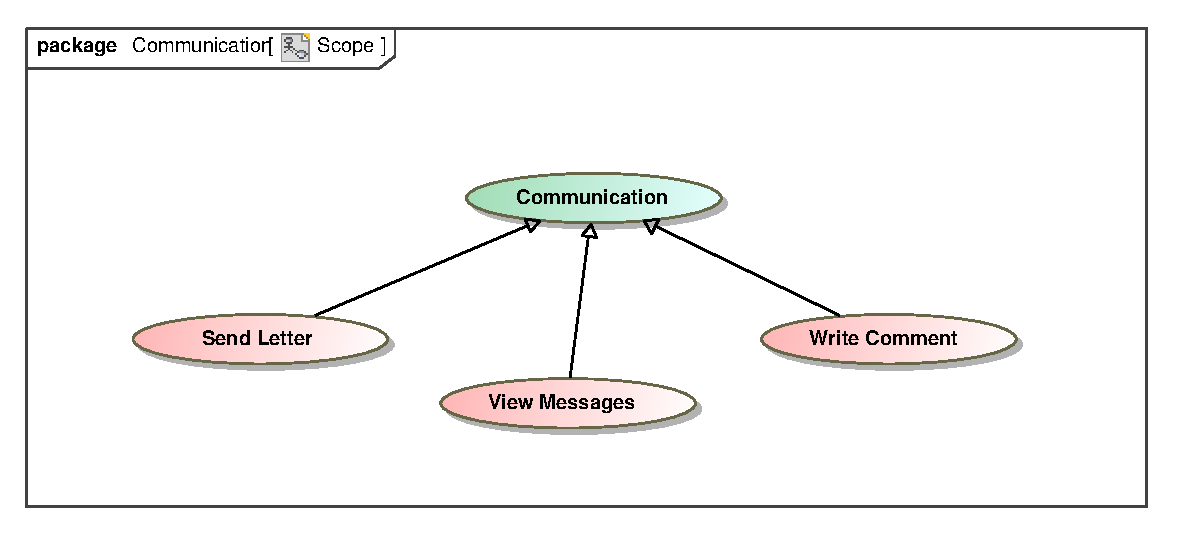
\includegraphics[scale=0.9]{epsImages/Communication/CommunicationScope.eps}
\caption{Scope of Communication module}
\end{figure}

\newpage
\subsubsection{Use Cases}

\begin{enumerate}
\item \textbf{Send Letter - priority: critical}
\par{This use case allows the writing and sending of an appropriate letter/message to the corresponding user, such as a query letter from author to agent. Available letters are: editorial letter, contract offer and query letter}

\begin{figure}[h]
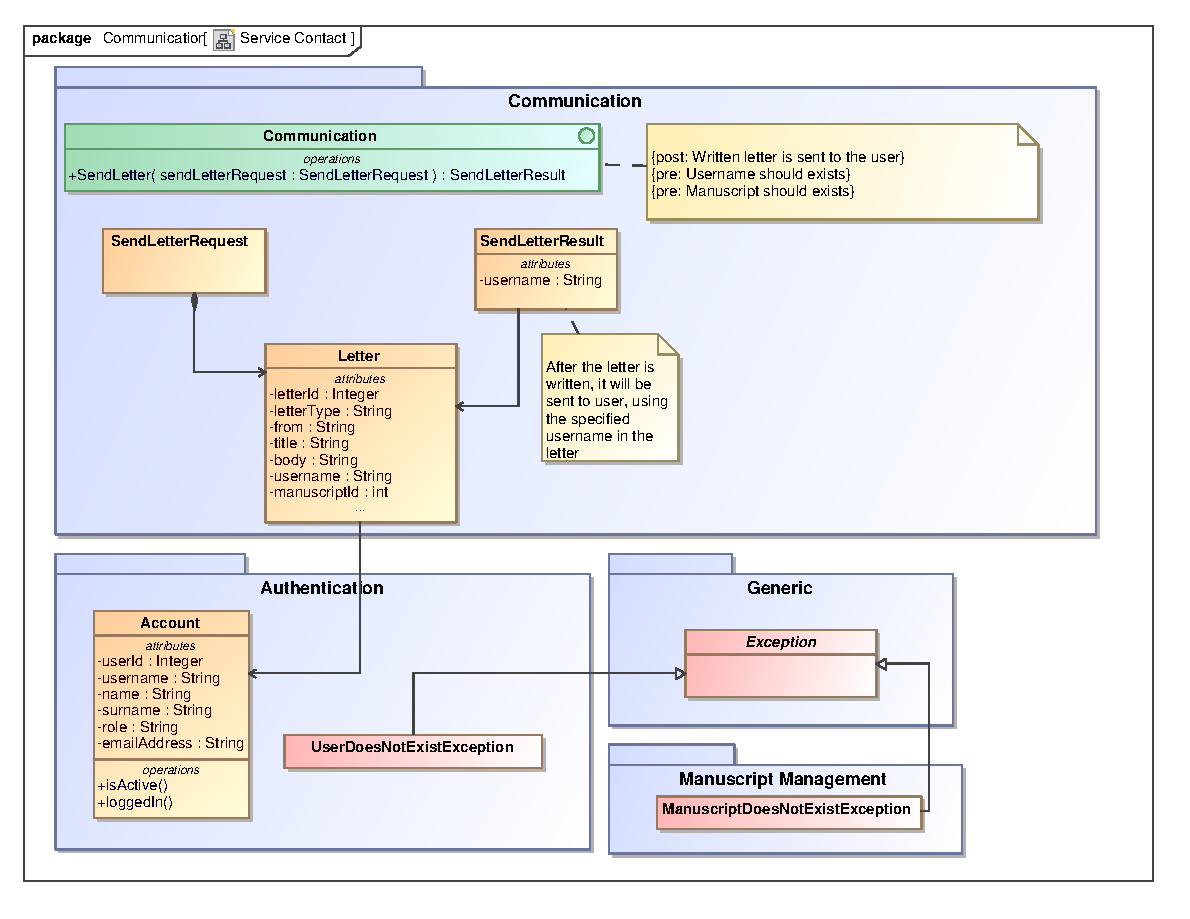
\includegraphics[scale=0.9]{epsImages/Communication/sendLetterServiceContract.eps}
\caption{Service contract for sending a letter}
\end{figure}

\newpage
\item \textbf{View Letter - priority: critical}\\
\par{This use case allows a user to view one of the letters sent to him/her. The letter can be an editorial letter, contract offer or query letter }\\ \\

\textbf{service contract:}

\begin{figure}[h]
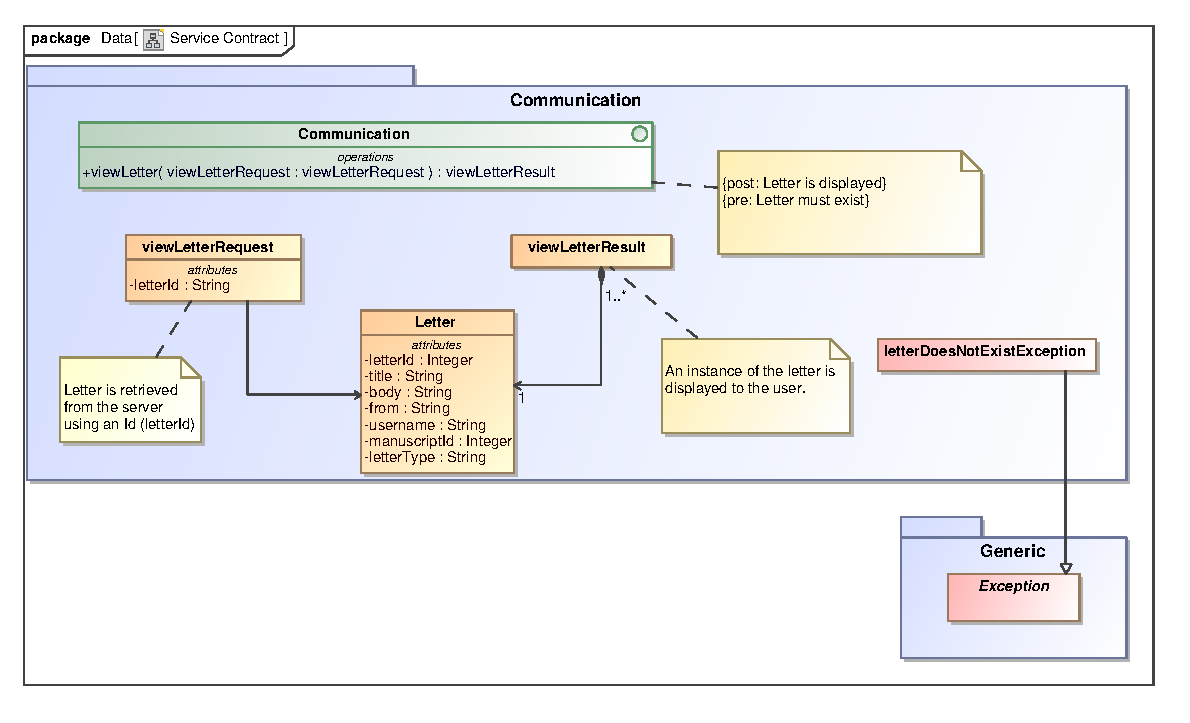
\includegraphics[scale=0.9]{epsImages/Communication/viewLetterServiceContract.eps}
\caption{Service contract for viewing a letter}
\end{figure}

\newpage

\item \textbf{Write Comment priority: nice to have}\\
\par{This allows a user (with the editor role) to add comments on the manuscript. Comments can be little notes to the author to indicate what the editor was thinking about that portion of the manuscript.}

\begin{figure}[h]
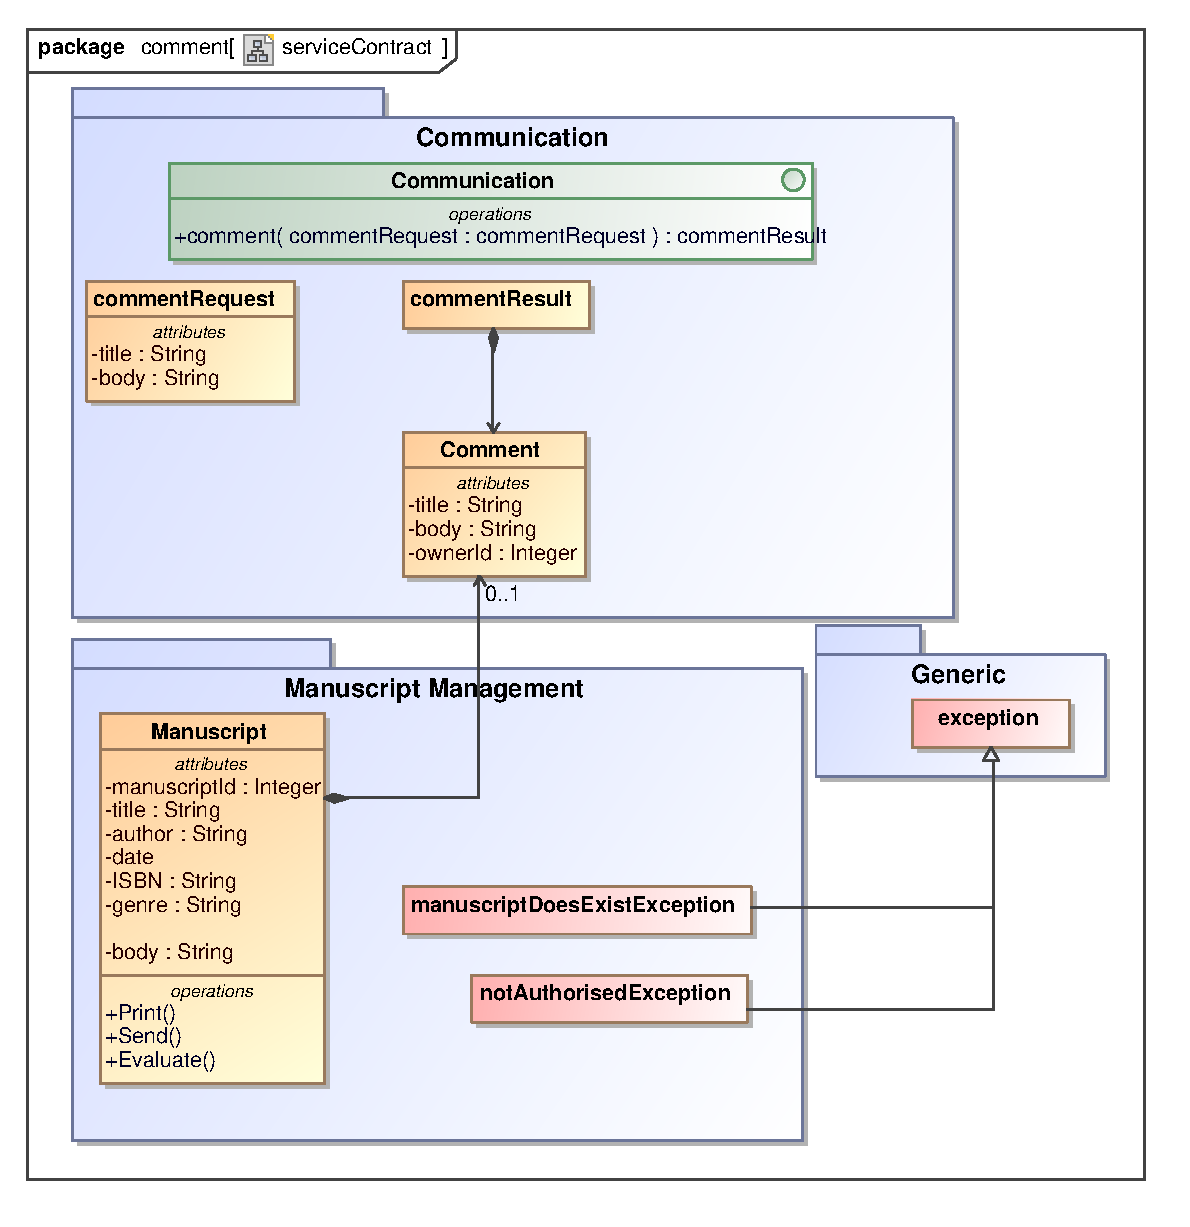
\includegraphics[scale=0.8]{epsImages/Communication/comment.eps}
\caption{Service contract for writing a comment a manuscript}
\end{figure}

\end{enumerate}
